Στο κεφάλαιο αυτό παρουσιάζεται η μοντελοποίηση της κυκλοφορίας σε έναν εξιδανικευμένο κόλπο, όπου το ένα άκρο του είναι ανοιχτό (\lat{open-sea-boundary}), ενώ τα υπόλοιπα κλειστά (στεριά).

Ο κόλπος έχει εξιναδικευτεί ώστε να έχει κάτοψη ορθογωνίου, με σταθερό βάθος και άτριβο πυθμένα. Το μοντέλο περιγράφει τη διάδοση ενός παλιρροϊκού κύματος από την ανοιχτή θάλασσα και το κλειστό άκρο, στο οποίο προσπίπτει το κύμα, προκαλεί τέλεια ανάκλαση.
\subsection{Παλίρροια και παλιρροϊκή κυκλοφορία}
Το φαινόμενο της παλίρροιας αναφέρεται στην περιοδική κίνηση του νερού της θάλασσας και οφείλεται στην διαφορά των ελκτικών δυνάμεων του Ηλίου και της Σελήνης, στις διάφορες φάσεις της.
Ως παλίρροια αναφέρεται η περιοδική ανύψωση και ταπείνωση της στάθμης της θάλασσας και συνοδεύεται από το παλλιροϊκό ρεύμα, δηλαδή την οριζόντια κίνηση του νερού. Και οι δύο κινήσεις αποτελούν μέρη του ίδιου φαινομένου.

Η περιοδική ανύψωση και ταπείνωση της στάθμης της θαλάσσας είναι επί της ουσίας ένα μακρύ κύμα το οποίο διαδίδεται. Η περίοδος ενός τέτοιου κύματος είναι συγκρίσιμη με το χρόνο περιστροφής της γης, αφού η παλίρροια μπορεί να έχει περίοδο 6, 12, ακόμα και 24 ώρες, οπότε επηρεάζεται από αυτή. Για αυτό στις εξισώσεις ορμής είναι απαραίτητη η προσθήκη του όρου της δύναμης \cor, εφόσον το φαινόμενο εξελίσεται σε μεταξύ διαφορετικών γεωγραφικών πλατών.

Ένα μακρύ κύμα περιγράφεται από την εξίσωση 
\begin{equation}
    η = \dfrac{H}{2}\cos{(kx-ωt)}
\end{equation}
όπου $Η$ το πλάτος κύματος, $k=\dfrac{2π}{L}$ o κυματαριθμός, $ω=\dfrac{2π}{T}$ η κυκλική συχνότητα, $L$ το μήκος κύματος και $T$ η περίοδος.

\subsection{Εξισώσεις ρηχού στρώματος - \lat{SWE}}
Πολλοί τύποι ροών μπορούν να χαρακτηριστούν ως "ροές ρηχού στρώματος". Με τον όρο ροή δεν είναι απαραίτητη η παραπομπή μόνο σε ροή ύδατος. Ροές όπως η κυκλοφορία ατμοσφαιρικών μαζών, η παλίρροια, πλημυρικά ρέματα, η παράκτια κυκλοφορία, τα \lat{tsunamis} κ.ά., μπορούν να περιγραφούν με τις εξισώσεις ρηχού στρώματος. Το βασικό χαρακτηριστικό τέτοιων ροών είναι ότι η κλίμακα του βάθους είναι πολύ μικρότερη από την οριζόντια χαρακτηριστική κλίμακα.
\begin{equation}
    \dfrac{h}{L} \ll 1
\end{equation}

Επομένως το αν θα εμπίπτει μία ροή στην κατηγορία εξισώσεων ρηχού στρώματος έχει σχέση με τις γεωμετρικές διαστάσεις της ίδιας της ροής και όχι του ρευστού όγκου που εξετάζεται. Για παράδειγμα η παλιρροϊκή ροή σε έναν ωκεανό περιγράφεται από τις εξισώσεις ρηχού στρώματος, όμως η ανεμογενής κυκλοφορία σε έναν ταμιευτήρα όχι, παρόλο που το βάθος του ταμιευτήρα είναι πολύ μικρό.

Στο μοντέλο του ρηχού στρώματος υπεισέρχεται η βασική απλοποιήση ότι η κατακόρυφη συνιστώσα της ταχύτητας, οπότε και της επιτάχυνσης είναι αμελητέες. Έτσι, η κατακόρυφη εξίσωση ορμής αποτελείται από υδροστατική ισορροπία.

Το σύστημα των διαφορικών εξισώσεων που περιγράφουν το πρόβλημα είναι οι εξισώσεις ορμής \lat{Navier - Stokes} και η εξίσωση συνέχειας. Ύστερα από ανάλυση της κλίμακας κάθε όρου των εξισώσεων και απαλοιφής των ασήμαντων, λόγω κλίμακας, όρων οι εξισώσεις ορμής για τους άξονες $x$, $y$, $z$ είναι αντίστοιχα
\begin{align}
    \dfrac{\partial{u}}{\partial{t}} + u\dfrac{\partial{u}}{\partial{x}} + v\dfrac{\partial{u}}{\partial{y}} + w\dfrac{\partial{u}}{\partial{z}} &= fv-\dfrac{1}{ρ}\dfrac{\partial{p}}{\partial{x}} + \dfrac{\partial}{\partial{z}}\left(ε_z\dfrac{\partial{u}}{\partial{z}}\right) \\
    \dfrac{\partial{v}}{\partial{t}} + u\dfrac{\partial{v}}{\partial{x}} + v\dfrac{\partial{v}}{\partial{y}} + w\dfrac{\partial{v}}{\partial{z}} &= fv-\dfrac{1}{ρ}\dfrac{\partial{p}}{\partial{y}} + \dfrac{\partial}{\partial{z}}\left(ε_z\dfrac{\partial{v}}{\partial{z}}\right) \\
    0 &= -\dfrac{1}{ρ}\dfrac{\partial{p}}{\partial{z}} - g
\end{align}
Το σύστημα συμπληρώνεται με την εξίσωση συνέχειας
\begin{equation}
    \dfrac{\partial{u}}{\partial{x}} + \dfrac{\partial{v}}{\partial{y}} + \dfrac{\partial{w}}{\partial{z}} = 0
\end{equation}

Η ύπαρξη ελεύθερης επιφάνειας του νερού εισάγει έναν ακόμα άγνωστο στο πρόβλημα της κυκλοφορίας. Η ανάπτυξη οποιουδήποτε ρεύματος συνεπάγεται τη μετατόπιση της ελεύθερης επιφάνειας από τη θέση ισορροπίας της, με αποτέλεσμα το πεδίο ορισμού της λύσης να είναι άγνωστο.

Ένας τρόπος αντιμετώσης αυτού του προβλήματος είναι να δημιουργήσουμε μία εξίσωση που να περιγράφει την θέση της ελεύθερης επιφάνειας κάθε χρονική στιγμή. Για το λόγο αυτό ολοκληρώνεται ως προς το βάθος η εξίσωση συνέχειας.

Έστω ότι με $ζ(t, x, y)$ συμβολίζεται το τοπικό βάθος της υδάτινης μάζας. Τότε η ολοκληρωμένη ως προς το βάθος εξίσωση συνέχειας δίνει
\begin{equation}
    \dfrac{\partial{ζ}}{\partial{t}} + \dfrac{\partial}{\partial{x}}\left(ζU\right) + \dfrac{\partial}{\partial{y}}\left(ζV\right) = 0 \label{eq:int-cont}
\end{equation}
όπου $U$ και $V$ οι μέσες ως προς το βάθος τιμές των $u$ και $v$ αντίστοιχα.

Ακόμα ολοκληρώνοντας την υδροστατική εξίσωση ως προς το βάθος, καταλήγουμε
\begin{align}
    -\dfrac{1}{ρ}\dfrac{\partial{p}}{\partial{x}} &= -g\dfrac{\partial{η}}{\partial{x}}-\dfrac{1}{ρ}\dfrac{\partial{p_α}}{\partial{x}} \\
    -\dfrac{1}{ρ}\dfrac{\partial{p}}{\partial{y}} &= -g\dfrac{\partial{η}}{\partial{y}}-\dfrac{1}{ρ}\dfrac{\partial{p_α}}{\partial{y}}
\end{align}

Μετά από τις κατάλληλες αντικαταστάσεις στο αρχικό σύστημα καταλήγουμε στις εξισώσεις ορμής, που μαζί με την ολοκληρωμένη ως προς το βάθος εξίσωση συνέχειας, αποτελούν τη βάση του μοντέλου ρηχού στρώματος
\begin{align}
    \dfrac{\partial{u}}{\partial{t}} + u\dfrac{\partial{u}}{\partial{x}} + v\dfrac{\partial{u}}{\partial{y}} + w\dfrac{\partial{u}}{\partial{z}} &= fv-g\dfrac{\partial{η}}{\partial{x}}-\dfrac{1}{ρ}\dfrac{\partial{p_α}}{\partial{x}} + \dfrac{\partial}{\partial{z}}\left(ε_z\dfrac{\partial{u}}{\partial{z}}\right) \label{eq:u-mom-non}\\
    \dfrac{\partial{v}}{\partial{t}} + u\dfrac{\partial{v}}{\partial{x}} + v\dfrac{\partial{v}}{\partial{y}} + w\dfrac{\partial{v}}{\partial{z}} &= fv-g\dfrac{\partial{η}}{\partial{y}}-\dfrac{1}{ρ}\dfrac{\partial{p_α}}{\partial{y}} + \dfrac{\partial}{\partial{z}}\left(ε_z\dfrac{\partial{v}}{\partial{z}}\right) \label{eq:v-mom-non}
\end{align}

\subsubsection{Τελικό μοντέλο}
Το μοντέλο που εξετάζεται στην παρούσα διπλωματική είναι αρκετά απλοποιημένο και δεν είναι απαραίτητη η χρήση όλων των όρων των εξισώσεων. Οι μη γραμμικοί όροι στις παραπάνω εξισώσεις μεταθέτουν μεν την ορμή, χωρίς όμως να μεταβάλλουν την ολική τιμή της. Καθώς η κυκλοφορία καθορίζεται από την ισορροπία των δυνάμεων, η μορφή της διατηρείται και στη γραμμικοποιημένη μορφή των εξισώσεων. Ακόμα, θεωρούμε ότι ο πυθμένας του κόλπου είναι άτριβος, η ατμοσφαιρική πίεση είναι σταθερή σε όλη την κάτοψη, καθώς και η εξέλιξη του φαινομένου γίνεται στο ίδιο γεωγραφικό πλάτος, με αποτέλεσμα η δύναμη \cor να μην επηρεάζει τη λύση.

Με βάση όλες αυτές τις παραδοχές, οι εξισώσεις \ref{eq:u-mom-non}, \ref{eq:v-mom-non} και \ref{eq:int-cont} γίνονται
\begin{align}
    \dfrac{\partial{u}}{\partial{t}} &= -g\dfrac{\partial{η}}{\partial{x}} \label{eq:u} \\
    \dfrac{\partial{v}}{\partial{t}} &= -g\dfrac{\partial{η}}{\partial{y}} \label{eq:v}
\end{align}
\begin{equation}
    \dfrac{\partial{η}}{\partial{t}} + h\dfrac{\partial{U}}{\partial{x}} + h\dfrac{\partial{V}}{\partial{y}} = 0 \label{eq:int-cont-new}
\end{equation}

Μετά από παραγώγιση των εξισώσεων \ref{eq:u} και \ref{eq:v} ως προς $x$ και $y$ αντίστοιχα και παραγώγιση της \ref{eq:int-cont-new} ως προς $t$, καταλήγουμε στην εξίσωση κύματος
\begin{equation}
    \dfrac{\partial^2{η}}{\partial{t}^2} = gh\left( \dfrac{\partial^2{η}}{\partial{x}^2} + \dfrac{\partial^2{η}}{\partial{y}^2} \right) \label{eq:wave}
\end{equation}
η οποία είναι μια υπερβολική διαφορική εξίσωση της μορφής $\dfrac{\partial^2{\vec{u}}}{\partial{t}^2}=c^2 \nabla^2 \vec{u}$, με $\vec{u} = \vec{u}(x_1, x_2, ... , x_n)$ βαθμωτή συνάρτηση της οποίας οι τιμές αποτελούν τη μετατόπιση ενός κύματος. Γίνεται αμέσως φανερό ότι η ταχύτητα του κύματος είναι 
\begin{equation}
    c=\sqrt{gh} \label{eq:celerity}
\end{equation}

\subsection{Διακριτοποίση των εξισώσεων}
Η αριθμητική επίλυση του προβλήματος γίνεται διακριτοποιώντας τις εξισώσεις (\ref{eq:u}), (\ref{eq:v}) και (\ref{eq:wave}). Επηλέχθηκε να γίνει χρήση της μεθόδου \textit{πεπερασμένων διαφορών}, έναντι της μεθόδου πεπερασμένων στοιχείων, προς χάρη της απλότητάς της. Βασιζόμενοι στη λογική της απλότητας χρησιμοποιήθηκε ένα ρητό σχήμα, διακριτοποιώντας το χρόνο με πρόσω διαφορές και το χώρο με κεντρικές, όπως συνιθίζεται σε φαινόμενα μεταφοράς.

Έτσι η διακριτοποιημένη μορφή της εξίσωση κύματος (\ref{eq:wave}) είναι
\begin{equation}
    η_{i,j}^{n+1} = 2 η_{i,j}^{n} - η_{i,j}^{n-1} + \dfrac{c^2 Δt^2}{Δx^2}\left( η_{i+1,j}^{n} - 2 η_{i,j}^{n} + η_{i-1,j}^{n}\right) + \dfrac{c^2 Δt^2}{Δy^2}\left( η_{i,j+1}^{n} - 2 η_{i,j}^{n} + η_{i,j+1}^{n}\right) \label{eq:dis:wave-1}
\end{equation}
όπου $c$ είναι η ταχύτητα κύματος, όπως υπολογίζεται στην εξίσωση (\ref{eq:celerity}).

Για λόγους ευπαρουσίασης της εξίσωσης (\ref{eq:dis:wave-1}), συμβολίζουμε ως
\begin{align}
    H_{x} &= η_{i+1,j}^{n} - 2 η_{i,j}^{n} + η_{i-1,j}^{n} \\
    H_{y} &= η_{i,j+1}^{n} - 2 η_{i,j}^{n} + η_{i,j+1}^{n} \\
    C_{xs} &= \dfrac{c^2 Δt^2}{Δx^2} \label{eq:cour-x-s}\\
    C_{ys} &= \dfrac{c^2 Δt^2}{Δy^2} \label{eq:cour-y-s}
\end{align}
οπότε η (\ref{eq:dis:wave-1}) γίνεται
\begin{equation}
    η_{i,j}^{n+1} = 2 η_{i,j}^{n} - η_{i,j}^{n-1} + C_{xs} H_{x} + C_{ys} H_{y}
    \label{eq:dis:wave}
\end{equation}
Οι αριθμοί (\ref{eq:cour-x-s}) και (\ref{eq:cour-x-s}), είναι το τετράγωνο του αριθμού \lat{Courant} για κάθε μία από τις δύο διευθύνσεις.

Για τη διακριτοποίηση των διαφορικών εξισώσεων της ταχύτητας (\ref{eq:u}) και (\ref{eq:v}) έγινε χρήση του ίδιου σχήματος, επομένως οι διακριτοποιημένες εξισώσεις, χρησιμοποιώντας τον παραπάνω συμβολισμό είναι
\begin{align}
    u_{i,j}^{n+1} &= u_{i,j}^{n} - g \dfrac{Δt}{Δx^2}H_x \label{eq:dis:u}\\
    v_{i,j}^{n+1} &= v_{i,j}^{n} - g \dfrac{Δt}{Δy^2}H_y \label{eq:dis:v}
\end{align} 
\subsubsection{Ευστάθεια της λύσης}
Όπως κάθε ρητό σχήμα επίλυσης, έτσι και αυτό που αναπτύχθηκε παραπάνω, είναι απαραίτητη η ύπαρξη μιας σχέσης που συνδέει το χρονικό βήμα, με το χωρικό βήμα.

Σύμφωνα με τον περιορισμό \lat{Courant-Friedrichs–Lewy} (\textbf{\lat{CFL condition}}) το χρονικό βήμα πρέπει να έχει τιμή μικρότερη από ένα συγκεκριμένο χρονικό διάστημα ώστε η αριθμητική λύση μιας υπερβολικής διαφορικής εξίσωσης να συγκλίνει.

Η μορφή του περιορισμού \lat{CFL} έχει σχέση με το πεδίο ορισμού της εξίσωσης που πρόκειται να λυθεί. Στο πρόβλημα της κυκλοφορίας σε ένα κόλπο, η επίλυση γίνεται στις δύο οριζόντιες διαστάσεις $x$, $y$ και η υπόθεση είναι 
\begin{equation}
    C = c Δt \dfrac{Δx + Δy}{Δx Δy}
\end{equation}
που προέκυψε από πρόσθεση του αριθμού \lat{Courant} για κάθε διεύθυνση.

Από φυσική άποψη, ο περιορισμός \lat{CFL} αναφέρεται στο γεγονός ότι το χρονικό βήμα πρέπει να είναι μικρότερο από το χρόνο που χρειάζεται το κύμα για να διασχίσει ένα χωρικό βήμα. Όταν η επίλυση του κύματος γίνεται στη μία διάσταση, αρκεί $ C \le 1$. Στην περίπτωση όμως που η επίλυση γίνεται στις δύο διαστάσεις, όπως στην παρούσα διπλωματική εργασία, ο περιορισμός γίνεται πιο αυστηρός και πρέπει $ C \le \dfrac{1}{\sqrt{2}} $. Η αυστηρότητα του περιορισμού έγγυται στο γεγονός ότι όταν ένα κύμα κινείται υπό γωνία στο πλέγμα επίλυσης πρέπει να διανύσει τη διαγώνια απόσταση ενός κελιού. Αυτό συχνά αναφέρεται και ως \textit{αριθμητικό ιξώδες} ή \textit{αριθμητική διάχυση}.

Με βάση λοιπόν τα παραπάνω, υπάρχει ένας περιορισμός για το μέγιστο χρονικό βήμα που είναι δυνατό να χρησιμοποιηθεί κατά την επίλυση και αυτό έχει άμεση σχέση με το χωρικό βήμα που επιλέγεται σε κάθε διεύθυνση. Επομένως, με γνωστό $Δx$ και $Δy$, το χρονικό βήμα υπολογίζεται
\begin{equation}
    Δt = \sqrt{2}\dfrac{ΔxΔy}{Δx+Δy}
    \label{eq:timestep}
\end{equation}

\subsection{Διαδικασία επίλυσης}
Η επίλυση του προβλήματος γίνεται σε τρία βασικά στάδια, την αρχικοποίηση των μεταβλητών με τα δεδομένα του προβλήματος, τους βασικούς υπολογισμούς και, τέλος, την οπτικοποίηση των αποτελεσμάτων.

\subsubsection{Δεδομένα του προβλήματος}
Ο σκοπός αυτής της διπλωματικής, πέραν όσων αναφέρθηκαν στα προηγούμενα κεφάλαια, είναι να υπολογισθεί αριθμητικά και να παρουσιασθεί η κυκλοφορία σε έναν ανοιχτό από τη μία πλευρά κόλπο. Επιλέχθηκε οι διαστάσεις του κόλπου αυτού να είναι $25km$ σε πλάτος και $40km$ σε μήκος, ενώ το βάθος του να είναι σταθερό $50m$.

Τα ύδατα του κόλπου τη χρονική στιγμη $t=0$ βρίσκονται σε ηρεμία και η διαδικασία επίλυσης αρχίζει με τη διέγερση του ανοιχτού άκρου από ένα ημιτονοειδές κύμα πλάτους $40cm$. Πρέπει να τονισθεί ότι τα σημεία στο άκρο του κόλπου διεγείρονται όλα ταυτόχρονα, οπότε προσομοιάζεται ένα εξωτερικό κύμα που εισέχεται στον κόλπο κάθετα, όπως φαίνεται στο σχήμα \ref{fig:layout}.

\begin{figure}[]
	\centering
	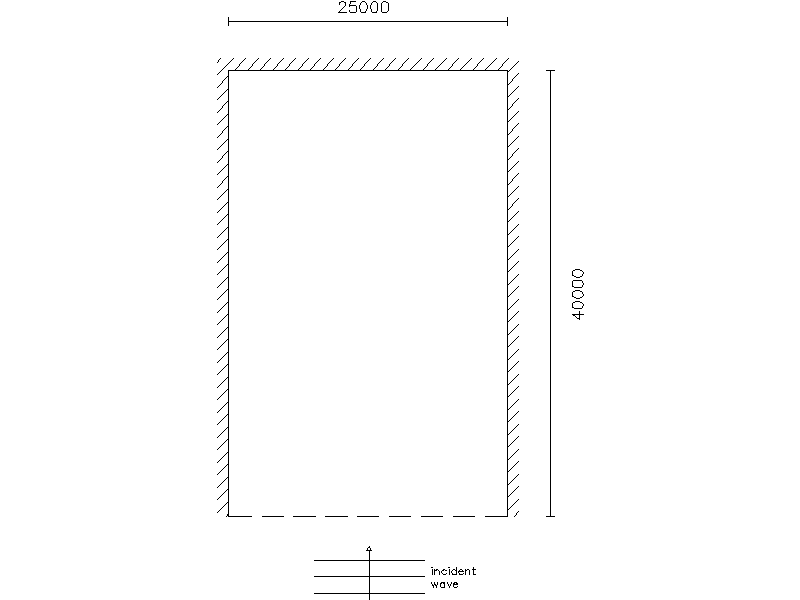
\includegraphics[scale=1.3]{images/layout.png}
	\caption{Κάτοψη του κόλπου. Με διακεκομένη γραμμή φαίνεται το ανοιχτό όριο.}
	\label{fig:layout}
\end{figure}

\begin{table}[h!]
    \centering
    \begin{tabular}{|l|r|l|r|}
        \hline
        \textbf{$L_x$} & $25km$ & \textbf{$T$} & $4000s$ \\
        \textbf{$L_y$} & $40km$ & \textbf{$A$} & $0.4m$ \\
        \textbf{$H$} & $50m$ & \textbf{$N_x$} & $50$ \\
        \textbf{$g$} & $9.807 m/s^2$ & \textbf{$N_y$} & $50$ \\
        \hline
    \end{tabular}
    \caption{Δεδομένα προβλήματος}
    \label{tab:in-data}
\end{table}

Στον Πίνακα \ref{tab:in-data} φαίνονται συγκεντρωμένα όλα τα δεδομένα του προβλήματος. Με $g$ συμβολίζεται η βαρυτική επιτάχυνση, ενώ με $N_x$ και $N_y$ ο αριθμός των κόμβων που επιλέχθηκαν για να δομήσουν το πλέγμα της επίλυσης. 

\subsubsection{Υπολογισμοί}
Οι υπολογισμοί για την επίλυση του προβλήματος διακρίνονται σε τρία στάδια.
\begin{itemize}
    \item Υπολογισμός χρονικού βήματος από την εξίσωση (\ref{eq:timestep})
    \item Για κάθε κόμβο του πλέγματος υπολογίζεται
    \begin{itemize}
        \item Η ανύψωση - ταπείνωση της ελεύθερης επιφάνειας $η$ από την εξίσωση (\ref{eq:dis:wave})
        \item Η οριζόντια ταχύτητα $u$ από την εξίσωση (\ref{eq:dis:u})
        \item Η κάθετη ταχύτητα $v$ από την εξίσωση (\ref{eq:dis:v})
    \end{itemize}
    \item Μεταβολή του χρόνου κατά $dt$ και επανάληψη του προηγούμενου βήματος
\end{itemize}

Ο προγραμματισμός της μεθόδου επίλυσης έγινε σε περιβάλλον \textit{Python} και το αντίστοιχο κομμάτι κώδικα φαίνεται στο παράρτημα \ref{sec:waterLevelPython} που υπολογίζεται η ανύψωση και ταπείνωση της ελεύθερης επιφάνειας, ενώ ο υπολογισμός της ταχύτητας φαίνεται στο παράρτημα \ref{sec:velocityPython}.

\subsubsection{Αρχικές και Συνοριακές συνθήκες}
Ο κόλπος πριν διεγερθεί από το εξωτερικό κύμα βρίσκεται σε κατάσταση ηρεμίας. Άρα οι αρχικές συνθήκες του προβλήματος είναι προφανές ότι θα είναι $0$ για την ανύψωση της ελεύθερης επιφάνειας, αλλά και για την ταχύτητα.
Η δυσκολία βρίσκεται στην εκλογή κατάλληλων συνοριακών συνθηκών, τέτοιων ώστε να προσομοιώνεται όσο το δυνατόν καλύτερα το πρόβλημα, με τους περιορισμούς που έχουμε θέσει.

Τα κλειστά άκρα του κόλπου (στεριά) προκαλούν πλήρη ανάκλαση των κυματισμών. Επομένως η επιλογή μία συνθήκης τύπου \lat{Neumann} είναι η πιο κατάλληλη. Για να υπάρχει πλήρης ανάκλαση των κυματισμών είναι απαραίτητο να μηδενίζεται η κλίση της ανύψωσης - ταπείνωσης της ελεύθερης επιφάνειας του νερού και όχι να μηδενίζεται η ίδια η τιμή της. Το ίδιο συμβαίνει και με την ταχύτητα. Επομένως οι συνοριακή συνθήκη για τα κλειστά άκρα του κόλπου είναι
\begin{align}
    \dfrac{\partial{η}}{\partial{x}} = \dfrac{\partial{η}}{\partial{y}} &= 0 \\
    \dfrac{\partial{u}}{\partial{x}} = \dfrac{\partial{v}}{\partial{y}} &= 0
\end{align}
Η εφαρμογή των παραπάνω συνθηκών έγινε προγραμματιστικά με την εισαγωγή \textit{κόμβων-φαντασμάτων} όπου η τιμή τους αυτόματα παίρνει την τιμή του προηγούμενου κόμβου. Έτσι, η διαφορά τους είναι $0$ και η κλίση του διανύσματος είναι, επίσης, $0$.

Για το ανοιχτό άκρο η εκλογή μια συνοριακής συνθήκης είναι πιο περίπλοκη, γιατί υπάρχει το προσπίπτων κύμα που μπαίνει στον κόλπο, αλλά και τα ανακλανόμενα κύματα που εξέρχονται από τον κόλπο. Το πρόβλημα είναι δυνατόν να λυθεί με χρήση της \textit{ελεύθερης ακτινοβολίας} που προτείνει ο \cite{koutitas}.
\begin{equation}
    \dfrac{\partial{ζ_r}}{\partial{t}} + \sqrt{gh} \dfrac{\partial{ζ_r}}{\partial{y}} = 0 
\end{equation}
η διακριτοποιήση της οποίας ακολουθεί το ίδιο σχήμα με τη διακριτοποίηση της ανύψωσης της ελεύθερης επιφάνειας, με πρόσω διαφορές στο χρόνο και κεντρικές διαφορές στο χώρο.
\begin{equation}
    ζ_{i,j}^{n+1} = 2 ζ_{i,j}^{n} - ζ_{i,j}^{n-1} + gh\dfrac{Δt^2}{2Δy^2}\left( ζ_{i+1,j}^{n} - 2ζ_{i,j}^{n} + ζ_{i,j+1}^{n} \right)
\end{equation}

\subsection{Αποτελέσματα επίλυσης}
Η επίλυση έγινε για διάφορες χρονικές περιόδους και αριθμό κόμβων, ώστε να διαπιστωθεί η ευστάθεια της μεθόδου. Σαν οπτικό αποτέλεσμα για κάθε επίλυση, το πρόγραμμα επιστρέφει μία σειρά διαγραμμάτων. Μία κάτοψη του κόλπου που εμφανίζεται η ελεύθερη επιφάνεια μαζί με τα διανύσματα της ταχύτητας για την τελευταία χρονική στιγμή της επίλυσης και δύο διαγραμμάτα χρονοσειράς για τη μεταβολή της ελεύθερης επιφάνειας και τη μεταβολή της κατά $y$ ταχύτητας ενός συγκεκριμένου σημείου κατά τη διαδικασία επίλυσης, δηλαδή για όλες τις χρονικές στιγμές.

\begin{table}[h!]
    \begin{tabular}{|cccccc||ccc|}
    \hline
    \multicolumn{2}{|c}{\textbf{\begin{tabular}[c]{@{}l@{}}Κωδικός\\ Επίλυσης\end{tabular}}} & \textbf{\begin{tabular}[c]{@{}c@{}}Χρονική \\ διάρκεια\end{tabular}} & \textbf{$N_x$} & \textbf{$N_y$} & \textbf{Σημείο} & \textbf{$Δx$ [m]} & \textbf{$Δy$ [m]} & \textbf{$Δt$ [s]} \\ \hline
    \multirow{2}{*}{1} & a & 0.5d & 50 & 50 & μέσο αν. ορίου & 500 & 800 & 30 \\
     & b & 0.5d & 50 & 50 & κέντρο κόλπου & 500 & 800 & 30 \\
    \multirow{2}{*}{2} & a & 0.5d & 25 & 25 & μέσο αν. ορίου & 1000 & 1600 & 39\\
     & b & 0.5d & 25 & 25 & κέντρο κόλπου & 1000 & 1600 & 39 \\ \hline
    \multirow{2}{*}{3} & a & 1d & 50 & 50 & μέσο αν. ορίου & 500 & 800 & 30 \\
     & b & 1d & 50 & 50 & κέντρο κόλπου & 500 & 800 & 30 \\
    \multirow{2}{*}{4} & a & 1d & 25 & 25 & μέσο αν. ορίου & 1000 & 1600 & 39\\
     & b & 1d & 25 & 25 & κέντρο κόλπου & 1000 & 1600 & 39 \\ \hline
    \multirow{2}{*}{5} & a & 5d & 25 & 25 & μέσο αν. ορίου & 1000 & 1600 & 39 \\
    & b & 5d & 25 & 25 & κέντρο κόλπου & 1000 & 1600 & 39 \\ \hline
    \end{tabular}
    \caption{Διαφορετικές επιλύσεις του προβλήματος}
    \label{tab:result-table}
\end{table}
Στον Πίνακα \ref{tab:result-table} φαίνονται οι διαφορετικές επιλύσεις που έγιναν για χρόνους επίλυσης $12 h$, $1 day$ και $5 days$, με διαφορετικό αριθμό κόμβων κάθε φορά. Ακόμα φαίνονται τα υπολογισμένα μεγέθη $Δx$, $Δy$ και $Δt$.

\subsubsection{Διαγράμματα επιλύσεων}
\begin{figure}[h]
	\centering
	\subfigure[Διάγραμμα Ε.Ε. και ταχύτητας]{\label{fig:1aF}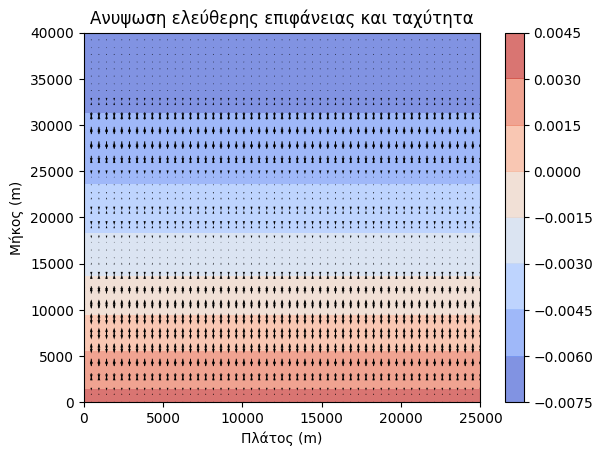
\includegraphics[scale=0.8]{1afinal_2d}}
	\subfigure[Διάγραμμα ταχύτητας σε κάτοψη]{\label{fig:1aV2d}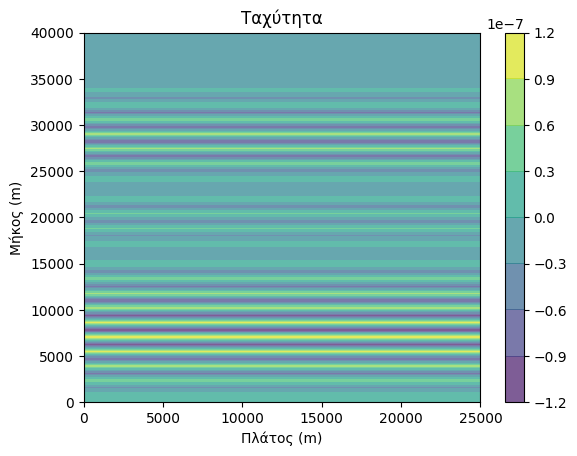
\includegraphics[scale=0.8]{1acontour}}
	\caption{Αποτελέσματα \lat{1a}}
\end{figure}
\begin{figure}[h]
	\centering
	\subfigure[Διάγραμμα Ε.Ε. και ταχύτητας]{\label{fig:1bF}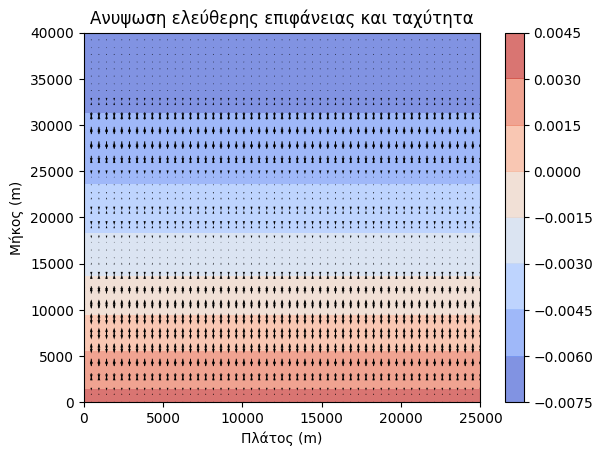
\includegraphics[scale=0.8]{1bfinal_2d}}
	\subfigure[Διάγραμμα ταχύτητας σε κάτοψη]{\label{fig:1bV2d}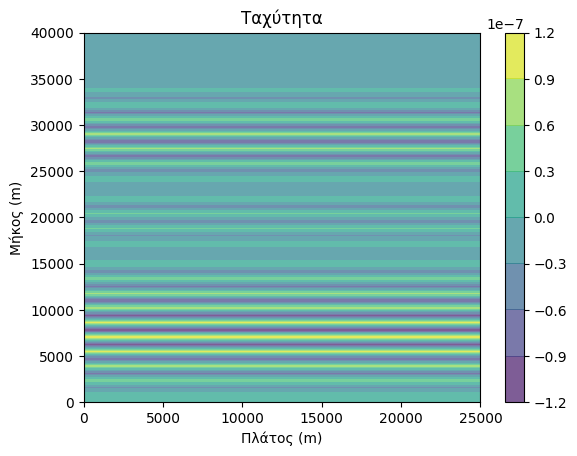
\includegraphics[scale=0.8]{1bcontour}}
	\caption{Αποτελέσματα \lat{1b}}
\end{figure}
\begin{figure}[h]
	\centering
	\subfigure[Διάγραμμα Ε.Ε. και ταχύτητας]{\label{fig:2aF}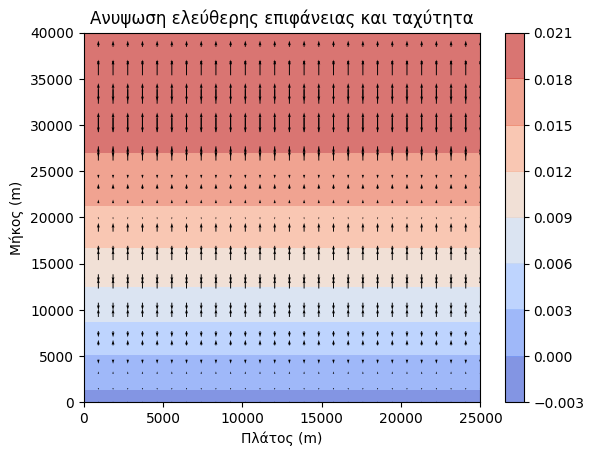
\includegraphics[scale=0.8]{2afinal_2d}}
	\subfigure[Διάγραμμα ταχύτητας σε κάτοψη]{\label{fig:2aV2d}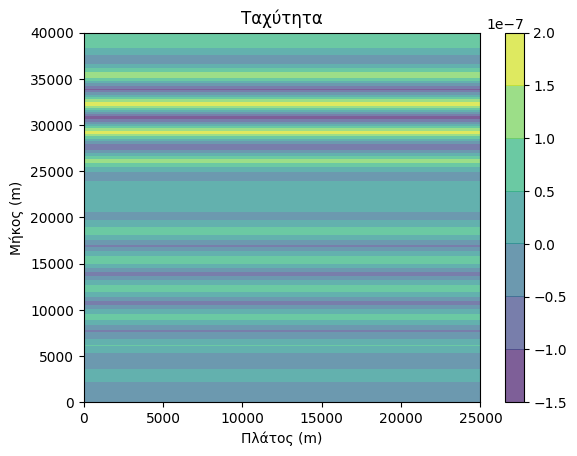
\includegraphics[scale=0.8]{2acontour}}
	\caption{Αποτελέσματα \lat{2a}}
\end{figure}
\begin{figure}[h]
	\centering
	\subfigure[Διάγραμμα Ε.Ε. και ταχύτητας]{\label{fig:2bF}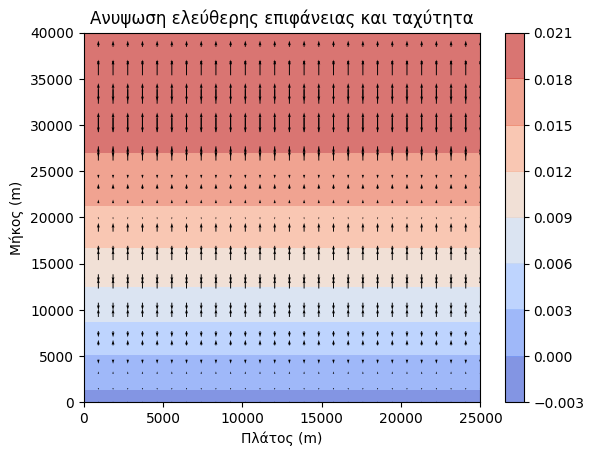
\includegraphics[scale=0.8]{2bfinal_2d}}
	\subfigure[Διάγραμμα ταχύτητας σε κάτοψη]{\label{fig:2bV2d}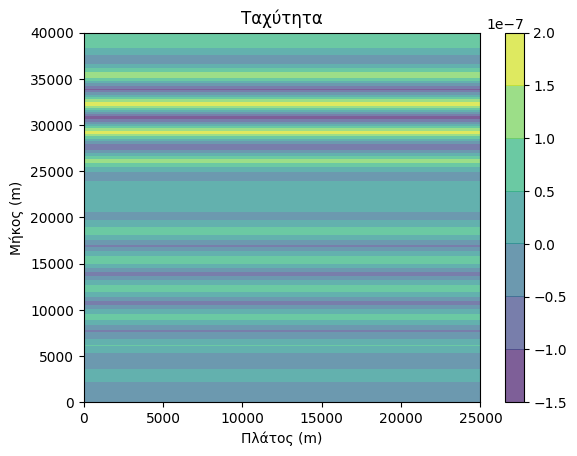
\includegraphics[scale=0.8]{2bcontour}}
	\caption{Αποτελέσματα \lat{2b}}
\end{figure}
\begin{figure}[h]
	\centering
	\subfigure[Διάγραμμα Ε.Ε. και ταχύτητας]{\label{fig:3aF}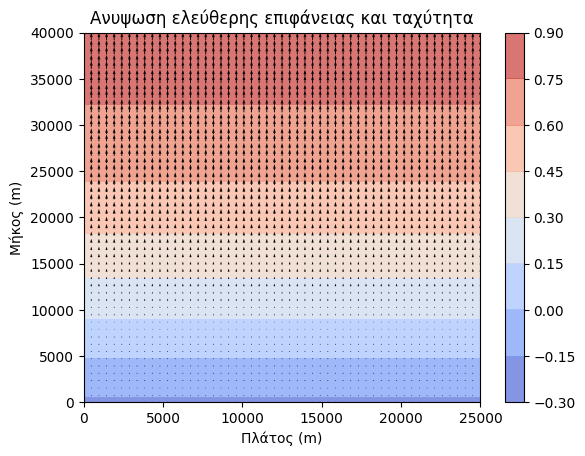
\includegraphics[scale=0.8]{3afinal_2d}}
	\subfigure[Διάγραμμα ταχύτητας σε κάτοψη]{\label{fig:3aV2d}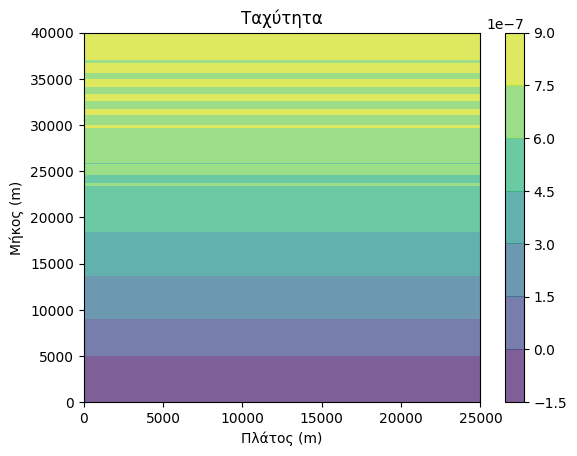
\includegraphics[scale=0.8]{3acontour}}
	\caption{Αποτελέσματα \lat{3a}}
\end{figure}
\begin{figure}[h]
	\centering
	\subfigure[Διάγραμμα Ε.Ε. και ταχύτητας]{\label{fig:3bF}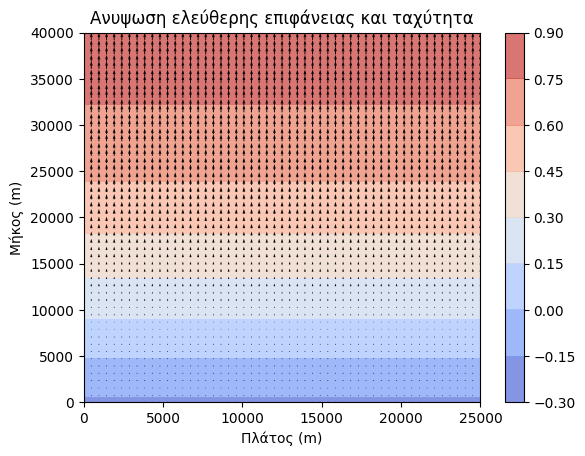
\includegraphics[scale=0.8]{3bfinal_2d}}
	\subfigure[Διάγραμμα ταχύτητας σε κάτοψη]{\label{fig:3bV2d}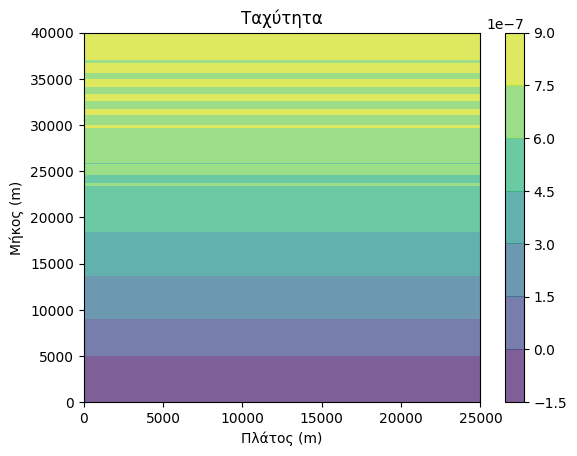
\includegraphics[scale=0.8]{3bcontour}}
	\caption{Αποτελέσματα \lat{3b}}
\end{figure}
\begin{figure}[h]
	\centering
	\subfigure[Διάγραμμα Ε.Ε. και ταχύτητας]{\label{fig:4aF}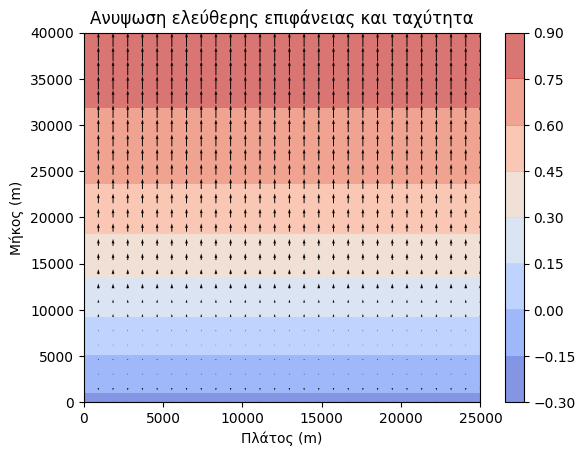
\includegraphics[scale=0.8]{4afinal_2d}}
	\subfigure[Διάγραμμα ταχύτητας σε κάτοψη]{\label{fig:4aV2d}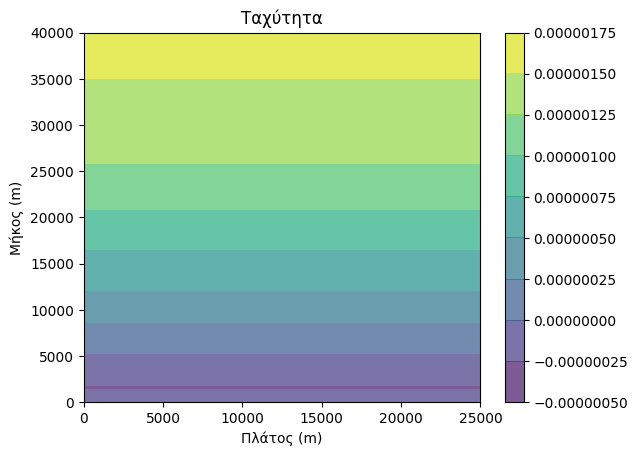
\includegraphics[scale=0.8]{4acontour}}
	\caption{Αποτελέσματα \lat{4a}}
\end{figure}
\begin{figure}[h]
	\centering
	\subfigure[Διάγραμμα Ε.Ε. και ταχύτητας]{\label{fig:4bF}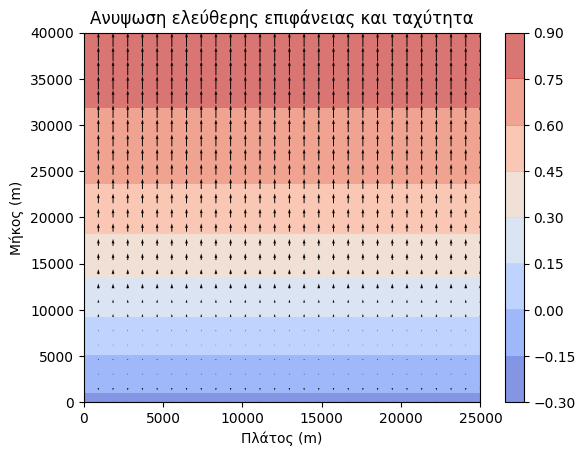
\includegraphics[scale=0.8]{4bfinal_2d}}
	\subfigure[Διάγραμμα ταχύτητας σε κάτοψη]{\label{fig:4bV2d}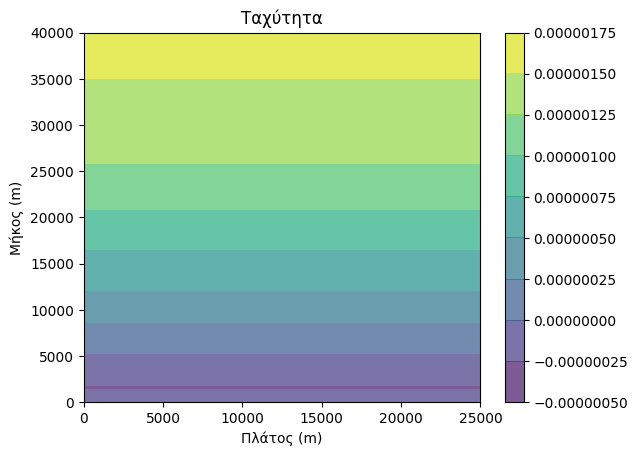
\includegraphics[scale=0.8]{4bcontour}}
	\caption{Αποτελέσματα \lat{4b}}
\end{figure}
\begin{figure}[h]
	\centering
	\subfigure[Διάγραμμα Ε.Ε. και ταχύτητας]{\label{fig:5aF}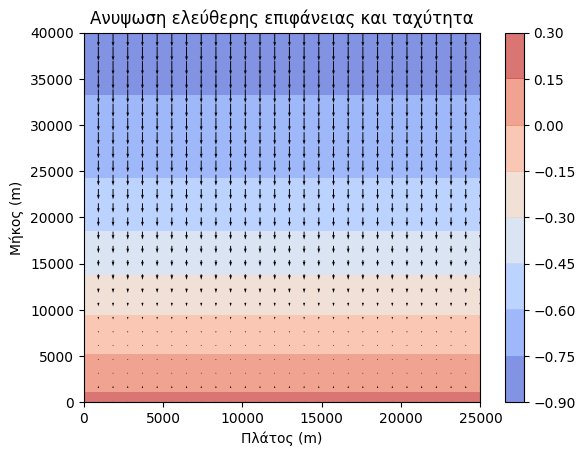
\includegraphics[scale=0.8]{5afinal_2d}}
	\subfigure[Διάγραμμα ταχύτητας σε κάτοψη]{\label{fig:5aV2d}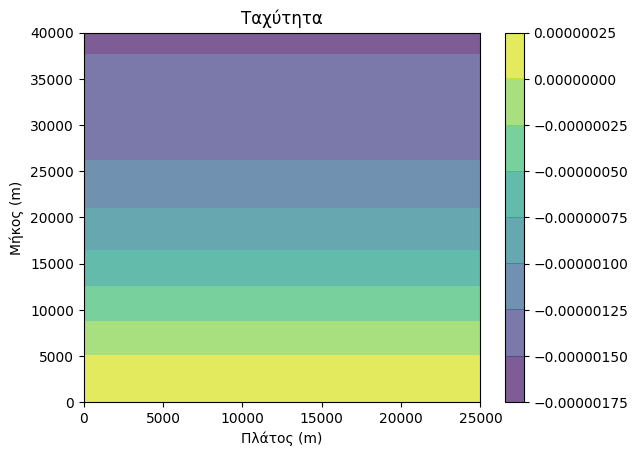
\includegraphics[scale=0.8]{5acontour}}
	\caption{Αποτελέσματα \lat{5a}}
\end{figure}
\begin{figure}[h]
	\centering
	\subfigure[Διάγραμμα Ε.Ε. και ταχύτητας]{\label{fig:5bF}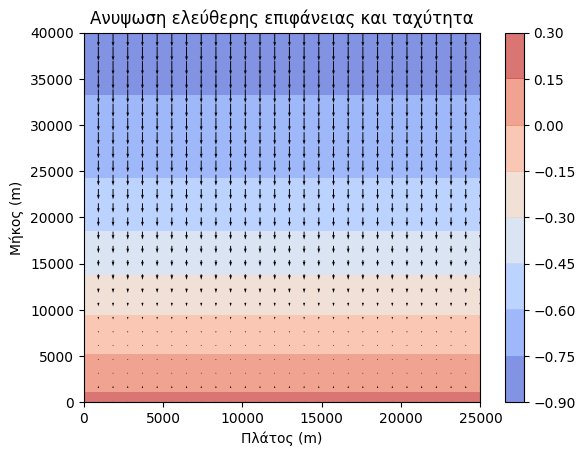
\includegraphics[scale=0.8]{5bfinal_2d}}
	\subfigure[Διάγραμμα ταχύτητας σε κάτοψη]{\label{fig:5bV2d}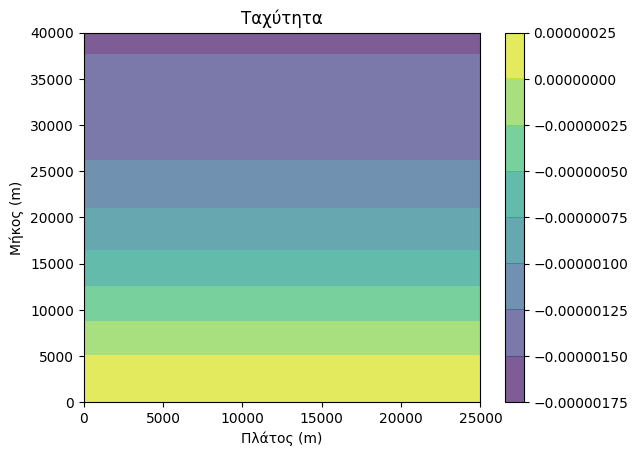
\includegraphics[scale=0.8]{5bcontour}}
	\caption{Αποτελέσματα \lat{5b}}
\end{figure}
\begin{figure}[h]
	\centering
	\subfigure[Χρονοσειρά ανύψωσης ελεύθερης επιφάνειας]{\label{fig:1a2aH}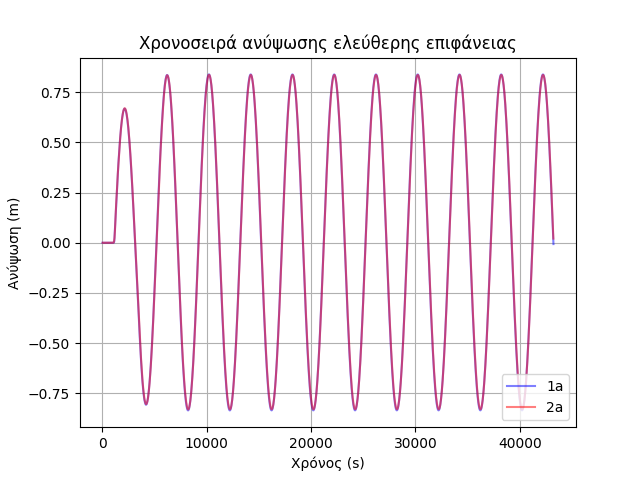
\includegraphics[scale=0.8]{1a2a-h}}
	\subfigure[Χρονοσειρά κατακόρυφης ταχύτητας]{\label{fig:1a2aV}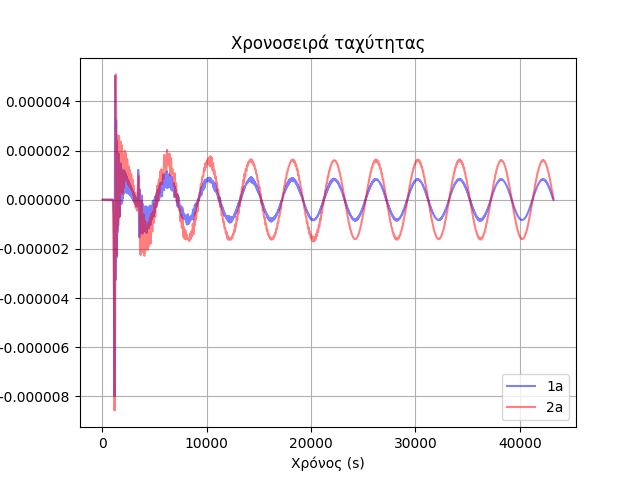
\includegraphics[scale=0.8]{1a2a-v}}
	\caption{Συγκριτικά αποτελέσματα χρονοσειρών 1a-2a}
\end{figure}
\begin{figure}[h]
	\centering
	\subfigure[Χρονοσειρά ανύψωσης ελεύθερης επιφάνειας]{\label{fig:1b2bH}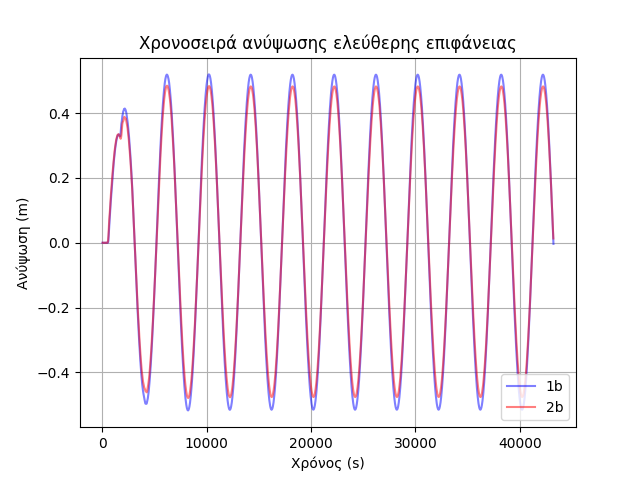
\includegraphics[scale=0.8]{1b2b-h}}
	\subfigure[Χρονοσειρά κατακόρυφης ταχύτητας]{\label{fig:1b2bV}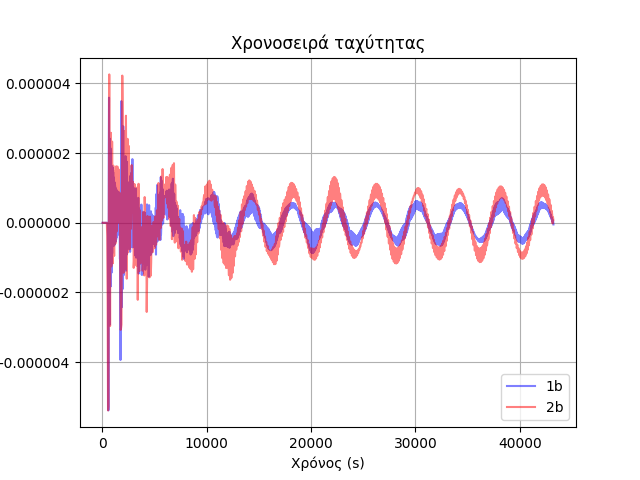
\includegraphics[scale=0.8]{1b2b-v}}
	\caption{Συγκριτικά αποτελέσματα χρονοσειρών 1b-2b}
\end{figure}
\begin{figure}[h]
	\centering
	\subfigure[Χρονοσειρά ανύψωσης ελεύθερης επιφάνειας]{\label{fig:3a4aH}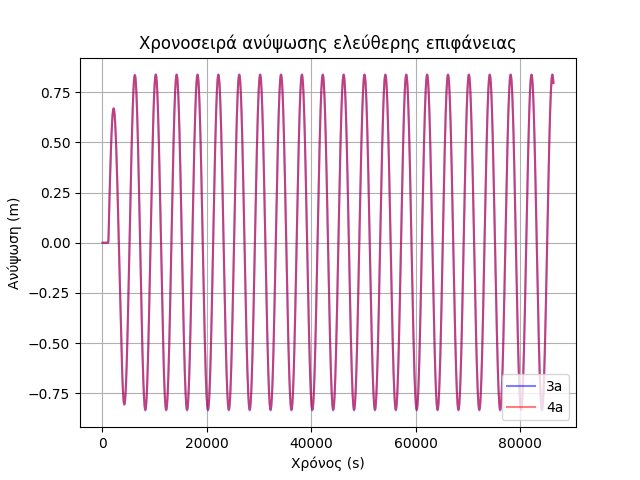
\includegraphics[scale=0.8]{3a4a-h}}
	\subfigure[Χρονοσειρά κατακόρυφης ταχύτητας]{\label{fig:3a4aV}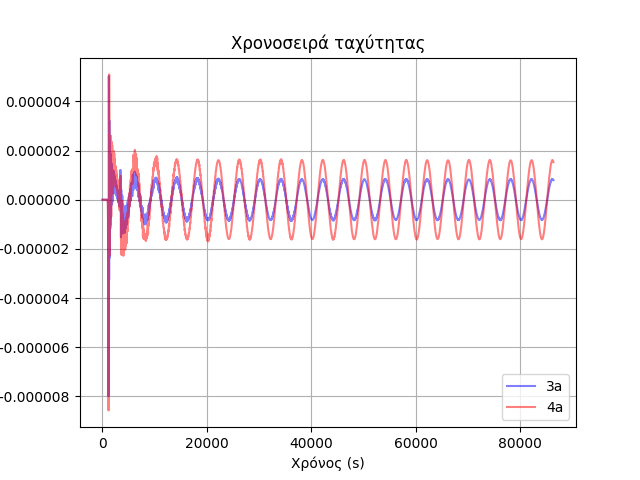
\includegraphics[scale=0.8]{3a4a-v}}
	\caption{Συγκριτικά αποτελέσματα χρονοσειρών 3a-4a}
\end{figure}
\begin{figure}[h]
	\centering
	\subfigure[Χρονοσειρά ανύψωσης ελεύθερης επιφάνειας]{\label{fig:3b4bH}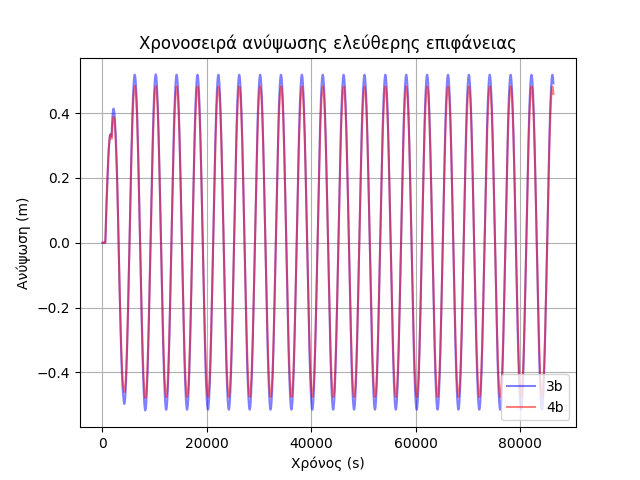
\includegraphics[scale=0.8]{3b4b-h}}
	\subfigure[Χρονοσειρά κατακόρυφης ταχύτητας]{\label{fig:3b4bV}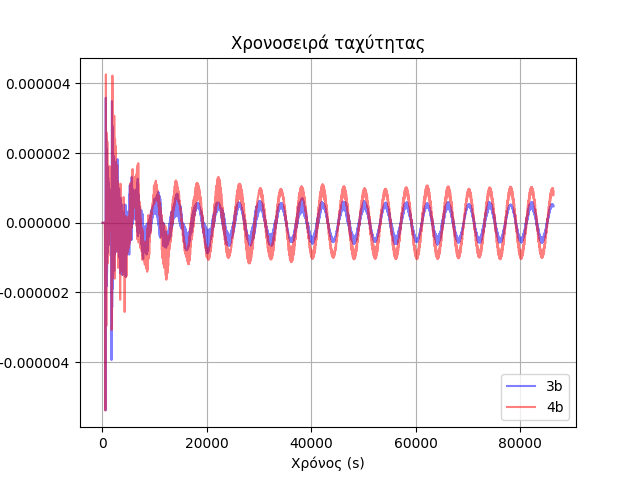
\includegraphics[scale=0.8]{3b4b-v}}
	\caption{Συγκριτικά αποτελέσματα χρονοσειρών 3b-4b}
\end{figure}

\cleardoublepage
\subsubsection{Σχολιασμός αποτελεσμάτων}
Τα αποτελέσματα από την παρουσίαση των διαγραμμάτων παρουσιάζουν ιδιαίτερο ενδιαφέρον. Όπως θα περίμενε κανείς όταν το πλέγμα γίνεται πιο πυκνό να υπάρχει μεγαύτερη ακρίβεια στον υπολογισμό των μεταβλητών του προβλήματος. Αντίθετα, φαίνεται, ότι κάτι τέτοιο δε συμβαίνει. Αυτό έγγυται στον περιορισμό \lat{CFL} που ανάλογα με το χωρικό βήμα αλλάζει αυτόματα και το χρονικό βήμα. Παρ' όλα αυτά, οι λύσεις συγκλίνουν και παρουσιάζουν συνοχή, ιδιαιτέρως σε μεγαλύτερους χρόνουν επίλυσης (1d, 5d).
Σε μεγάλους χρόνους επίλυσης, η ταχύτητα παρουσιάζει την αναμενόμενη συμπεριφορα, δηλαδή να κρατά σταθερό πρόσημο σε όλο το πλέγμα κάθε χρονική στιγμή, όπως φαίνεται από τα διαγράμματα \ref{fig:4aV2d}, \ref{fig:4bV2d}, \ref{fig:5aV2d} και \ref{fig:5bV2d}. 

Ενδιαφέρον παρουσιάζουν και τα διαγράμματα χρονοσειρών της ταχύτητας, καθώς παρατηρούμε το μεγάλο σφάλμα στον υπολογισμό για τις 2 πρώτες ώρες περίπου. Η λύση, όμως, ομαλοποιείται και λαμβάνει την αναμενόμενη ημιτονοειδή μορφή με το πέρασμα του χρόνου, όπου και σταθεροποιείται.

Όσον αφορά τα διαγράμματα χρονοσειράς της ανύψωσης της ελεύθερης επιφάνειας, παρατηρούμε ότι δημιουργείται στάσιμο κύμα πλάτους $2Α \approx 0.8m$, όπως φυσικά θα περίμενε κανείς, λόγω της πλήρους ανάκλασης.